\documentclass[11pt]{article}
\usepackage{amsmath,amssymb,amsthm}
\usepackage{geometry}
\usepackage{tikz}
\usepackage{xstring}
\usepackage{forest}
\usepackage{url}
\usepackage[hidelinks,bookmarks=false]{hyperref}
\geometry{margin=1in}
\setlength{\parindent}{0pt}
\setlength{\parskip}{1ex}

\newtheorem{lemma}{Lemma}
\newtheorem{theorem}{Theorem}
\newtheorem{corollary}{Corollary}
\newtheorem{remark}{Remark}

% \ShowGrid{<comma-separated cells>} draws the 3x3 grid as a compact array of
% dots, row-major (1..9 as in the Setup section): a small dot for each cell
% not in the list, a larger dot for each cell that is. Usable inline or in
% display math, e.g. \[ \left(\ShowGrid{2,5,9}\right)^a = \ShowGrid{5,4,9} \].
% (Note: \show is a plain TeX primitive and digits can't directly follow
% letters in a control word name, so this can't literally be spelled \show33.)
\newcommand{\GridSpacing}{3mm}
\newcommand{\GridDotSmall}{0.35mm}
\newcommand{\GridDotBig}{1.1mm}
\newcommand{\ShowGrid}[1]{%
  \begingroup
  \edef\marked{,#1,}%
  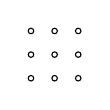
\begin{tikzpicture}[baseline=(current bounding box.center)]
    \foreach \i in {1,...,9} {
      \pgfmathtruncatemacro{\r}{int((\i-1)/3)}
      \pgfmathtruncatemacro{\c}{mod(\i-1,3)}
      \IfSubStr{\marked}{,\i,}{\edef\rad{\GridDotBig}\def\Mark{\fill}}{\edef\rad{\GridDotSmall}\def\Mark{\draw}}
      \Mark (\c*\GridSpacing,-\r*\GridSpacing) circle (\rad);
    }
  \end{tikzpicture}%
  \endgroup
}

% \ShowStrip{<comma-separated cells>} is \ShowGrid's analogue for the 2x4
% strip of Section 5: row-major cells 1..8, 4 per row.
\newcommand{\ShowStrip}[1]{%
  \begingroup
  \edef\marked{,#1,}%
  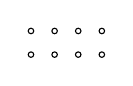
\begin{tikzpicture}[baseline=(current bounding box.center)]
    \foreach \i in {1,...,8} {
      \pgfmathtruncatemacro{\r}{int((\i-1)/4)}
      \pgfmathtruncatemacro{\c}{mod(\i-1,4)}
      \IfSubStr{\marked}{,\i,}{\edef\rad{\GridDotBig}\def\Mark{\fill}}{\edef\rad{\GridDotSmall}\def\Mark{\draw}}
      \Mark (\c*\GridSpacing,-\r*\GridSpacing) circle (\rad);
    }
  \end{tikzpicture}%
  \endgroup
}

% \SetupGrid draws the 3x3 grid as 9 labelled tiles with small clockwise-
% rotation icons at the centre of each of the four 2x2 blocks, for the
% illustration in the Setup section.
\newcommand{\SetupGrid}{%
  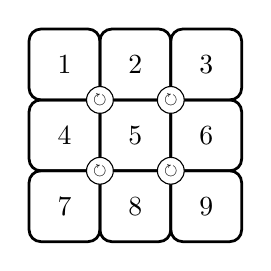
\begin{tikzpicture}[baseline=(current bounding box.center)]
    \def\tileSize{9mm}
    \def\tileGap{3mm}
    \def\step{\tileSize+\tileGap}
    \foreach \i in {1,...,9} {
      \pgfmathtruncatemacro{\r}{int((\i-1)/3)}
      \pgfmathtruncatemacro{\c}{mod(\i-1,3)}
      \node[rectangle, rounded corners=1.5mm, draw=black, line width=1pt,
            minimum width=\tileSize, minimum height=\tileSize,
            font=\normalsize] at (\c*\step,-\r*\step) {\i};
    }
    \foreach \r in {0,1} {
      \foreach \c in {0,1} {
        \node[circle, draw=black, fill=white, inner sep=0pt, minimum size=3.4mm]
          at ({(\c+0.5)*\step},{-(\r+0.5)*\step}) {\tiny$\circlearrowright$};
      }
    }
  \end{tikzpicture}%
}

% \EL{<label>} (as a forest key, "EL={<label>}") draws an arrow edge in a
% forest tree labelled by <label> in math mode, e.g. EL={c^{-1}}. Must be
% defined via \forestset (a plain \newcommand is invisible to forest's own
% key-value parser and corrupts the tree parse).
\forestset{
  EL/.style n args=1{edge label={node[midway,fill=white,inner sep=1pt,font=\scriptsize]{$#1$}}}
}

\title{Which Block-Rotation Puzzles Generate the Symmetric Group?}
\author{Michael Albert \\ University of Otago}
\date{}

\begin{document}
\maketitle

\begin{abstract}
For an $m\times n$ grid of cells, let $G_{m,n}$ be the group generated by clockwise $90^\circ$ rotations of all $2\times2$ blocks. We give an elementary, self-contained proof that, for $2 \le m \le n$, $G_{m,n}$ is the full symmetric group on the $mn$ cells if and only if $m \ge 3$ or $n \ge 4$ — avoiding classical primitivity arguments such as Jordan's theorem in favour of direct computations, the grid's own geometric symmetries, and a short exhaustive search. As a by-product, we show that the one interesting exceptional case, $G_{2,3}$, is isomorphic to $S_5$, realizing on this puzzle-derived set of $6$ points the classical exotic degree-$6$ representation of $S_5$.
\end{abstract}

\section{Introduction}

Consider this grid
\[
\SetupGrid
\]
and the question ``Which permutations of its cells can be achieved by rotating the four $2\times2$ corner blocks repeatedly?'' 

More formally, let $G \le S_9$ be the group generated by the four elements:
\[
a = (1\,2\,5\,4), \qquad b = (2\,3\,6\,5), \qquad c = (4\,5\,8\,7), \qquad d = (5\,6\,9\,8),
\]
with the goal being to understand the structure of $G$.\footnote{Spoilers: $G$ is the full symmetric group $S_9$, and the same holds for $m\times n$ grids for all $m,n \ge 3$ and also for $2\times n$ strips for $n \ge 4$.}

The corresponding group arose in a \href{https://michael-albert-dun.github.io/tintangle}{puzzle} that I was working on in the $4\times4$ case, which led me to this exploration. The result is not new — in fact, a more complete treatment can already be found in a paper by Lam \cite{Lam2022} — but the argument here is elementary, different, and self-contained.

First we'll show that $G$ contains a $3$-cycle. That's a standard step in ``block moving puzzles''. From that point, I could blind you with science \cite{Dolby1982}: \emph{it is easy to see that $G$ is $2$-transitive, hence primitive, so that Jordan's theorem \cite{DixonMortimer1996, Jordan1873} implies that $G$ is either $A_9$ or $S_9$; but the generators are odd, so only the latter is possible.}

However, in the spirit of the \href{https://michael-albert-dun.github.io/tintangle}{puzzle} that inspired this note in the first place, we'll give a more elementary argument that proves that \emph{all} $3$-cycles belong to $G$.

\section{A symmetry observation}\label{sec:symmetry}

The $3\times3$ grid carries an obvious geometric symmetry: the dihedral group $D_4$ of order $8$ (the four rotations and four reflections of the square) acts on the $9$ cells, and this action permutes the four $2\times2$ corner blocks among themselves. It therefore also acts, by conjugation, on the generating set $\{a,b,c,d\}$ — and a direct check shows this action follows the geometry exactly:

\begin{itemize}
\item the rotations of the grid permute $a,b,c,d$ amongst themselves, following the blocks around the centre: a $90^\circ$ clockwise rotation of the whole grid sends $a\mapsto b\mapsto d\mapsto c\mapsto a$, and a $180^\circ$ rotation swaps $a\leftrightarrow d$ and $b\leftrightarrow c$;
\item the four reflections send each generator to the \emph{inverse} of a generator, e.g.\ the reflection across the main diagonal fixes the blocks of $a$ and $d$ setwise but sends $a\mapsto a^{-1}$, $d\mapsto d^{-1}$, and swaps $b\mapsto c^{-1}$, $c\mapsto b^{-1}$.
\end{itemize}

The pattern is exactly orientation: an orientation-preserving symmetry of the plane turns a clockwise rotation of a block into a clockwise rotation of the image block, i.e.\ another generator, while an orientation-reversing symmetry turns a clockwise rotation into a counter-clockwise one, i.e.\ the inverse of a generator. In particular every element of $D_4$ conjugates $\{a,b,c,d\}$ back into $\{a^{\pm1},b^{\pm1},c^{\pm1},d^{\pm1}\} \subset G$, so $D_4$ normalizes $G$.

This lets us transfer any fact proved about the action on one collection of cells to its whole $D_4$-orbit for free, without repeating the underlying computation. 

\section{Creating all $3$-cycles}

In generating all $3$-cycles it suffices to generate a $3$-cycle of each possible support (the set of three points that it moves) since, if two $3$-cycles have the same support, each is the square of the other. So the plan is to transport supports of $3$-cycles around the grid using both conjugation by elements of the group itself, and the symmetry of the grid. We begin with a direct calculation that produces a $3$-cycle from the generators.
\[
a^{-1} d^{-1} a d  = (4\;5\;6).
\]

See \ref{app:single-point-overlaps} for a lemma that provides hints about where to hunt for initial $3$-cycles in puzzles of this type.

Beginning from our single $3$-cycle $(4\;5\;6)$, we will successively construct more $3$-cycles with different supports until we have one for every symmetry type of a triple of distinct cells.

For this purpose we use a simple graphical representation of $3$-element subsets of the $3\times3$ grid — for instance, the support of the $3$-cycle $(4\;5\;6)$ is represented as:

\[
\ShowGrid{4,5,6}
\]

There are $\binom{9}{3}=84$ $3$-element subsets of the grid. A direct check shows that up to the symmetry of $D_4$, there are exactly $16$ orbits: six of size $8$, eight of size $4$, and two of size $2$. One representative of each orbit is shown in the following table:

\[
\begin{array}{c|cccccc}
\text{orbits of size }8 & \ShowGrid{1,2,5} & \ShowGrid{1,2,6} & \ShowGrid{1,2,7} & \ShowGrid{1,2,8} & \ShowGrid{1,2,9} & \ShowGrid{1,5,6} \\[6mm]
\text{orbits of size }4 & \ShowGrid{1,2,3} & \ShowGrid{1,2,4} & \ShowGrid{1,3,5} & \ShowGrid{1,3,7} & \ShowGrid{1,3,8} & \ShowGrid{1,6,8} \\[6mm]
 & \ShowGrid{2,4,5} & \ShowGrid{2,4,6} & & & & \\[6mm]
\text{orbits of size }2 & \ShowGrid{1,5,9} & \ShowGrid{4,5,6} & & & &
\end{array}
\]

The last of these, $\{4,5,6\}$, is the support we already have. The task is to find, for each of the remaining $15$ shapes a way to reach it from $\{4,5,6\}$ by conjugation with elements of $G$. The tree below shows the results of such a search.

\begin{center}
\begin{forest}
  for tree={parent anchor=south, child anchor=north, l sep=9mm, s sep=3mm, edge={-latex}}
  [\ShowGrid{4,5,6}
    [\ShowGrid{1,4,6}, EL={a}
      [\ShowGrid{1,2,6}, EL={a}
        [\ShowGrid{1,3,5}, EL={b}]
      ]
      [\ShowGrid{1,4,5}, EL={b}
        [\ShowGrid{1,2,4}, EL={a}]
        [\ShowGrid{1,4,7}, EL={c^{-1}}]
      ]
      [\ShowGrid{1,5,6}, EL={c}
        [\ShowGrid{1,6,8}, EL={c}]
      ]
      [\ShowGrid{1,4,9}, EL={d}
        [\ShowGrid{1,5,9}, EL={c}]
        [\ShowGrid{1,7,9}, EL={c^{-1}}]
      ]
      [\ShowGrid{1,3,4}, EL={b^{-1}}]
      [\ShowGrid{1,6,7}, EL={c^{-1}}]
    ]
    [\ShowGrid{2,4,5}, EL={b}
      [\ShowGrid{2,4,6}, EL={d}]
    ]
  ]
\end{forest}
\end{center}

A representative of every one of the $16$ shapes from the catalog appears exactly once in this tree, so $G$ contains a $3$-cycle of every possible support and, as noted above, this is enough to conclude that $G$ contains every $3$-cycle in $S_9$.

The $3$-cycles generate $A_9$, so we now know that $A_9 \le G$. The generator $a = (1\;2\;5\;4)$ is a $4$-cycle, hence an odd permutation, so $a \notin A_9$. Since $A_9$ is a maximal subgroup of $S_9$,
\[
G = S_9. \qquad \blacksquare
\]

\section{Generalization to $m\times n$ grids}

The argument extends to non-square grids, as long as both dimensions are at least $3$.

\begin{theorem}\label{thm:mxn}
Let $m,n \ge 3$, and let $G_{m,n} \le S_{mn}$ be generated by the $(m-1)(n-1)$ rotations of the $2\times2$ blocks of an $m\times n$ grid. Then $G_{m,n} = S_{mn}$.
\end{theorem}
\begin{proof}
Any $3\times3$ block of consecutive rows and columns is itself a $3\times3$ grid whose four corner-rotation generators are among the generators of $G_{m,n}$; by the previous results, that block's local group is the full symmetric group on its $9$ cells, fixing everything outside it. Every grid-adjacent pair of cells lies inside some such $3\times3$ block so $G_{m,n}$ contains every adjacent transposition. The grid's adjacency graph is connected, and transpositions indexed by the edges of such a graph generate the full symmetric group on its vertices, so $G_{m,n}=S_{mn}$.
\end{proof}

\section{The $2\times n$ strip}

For completeness, consider the case $m=2$, a grid with two rows. Label the $2\times n$ grid with cells $1,\dots,n$ in the top row, and $n{+}1,\dots,2n$ in the bottom row, and let $G_n \le S_{2n}$ be generated by the $n-1$ block rotations
\[
g_i = (i\;\,i{+}1\;\,i{+}n{+}1\;\,i{+}n), \qquad i = 1,\dots,n-1.
\]

\subsection*{$n=2$: Too small to matter}
$G_2 = \langle g_1\rangle$ is cyclic of order $4$, far short of $|S_4|=24$.

\subsection*{$n=3$: Proper, by direct computation}
Direct computation gives $|G_3| = 120 < 720 = |S_6|$, so $G_3 \neq S_6$. In fact $G_3$ is isomorphic to $S_5$, as is proved in \ref{app:g3iso}.

\subsection*{$n=4$: Full, via symmetry and a short search}

Adjacent generators of the strip overlap in \emph{two} points, not one, so Lemma~\ref{lem:onepoint} does not apply to $g_1,g_2$ to give a $3$-cycle directly. However, 

\begin{lemma}\label{lem:strip3cycle}
$G_4$ contains the $3$-cycle $(2\;3\;4)$.
\end{lemma}
\begin{proof}
A direct check of the product gives
\[
[g_1,g_2] = (2\;3)(5\;6),
\]
a double transposition, and this \emph{does} share exactly one moved point (3) with $g_3$. Lemma~\ref{lem:onepoint} applies to $\sigma=[g_1,g_2]$, $\tau=g_3$ giving $[\sigma,\tau]=(2\;3\;4)$.
\end{proof}

The $2\times4$ strip is not square, so it has no $90^\circ$ rotational symmetry — only the Klein four-group $V_4=\{e,h,v,hv\}$ of order $4$, where $h$ is the left-right mirror and $v$ is the top-bottom mirror of the strip. But we are free to use this more limited group of symmetries to sweep the $3$-cycle $(2\;3\;4)$ around the strip.

So first we need to find representatives of all the possible triples. Here, each orbit has size four since none of the non-identity elements of $V_4$ can fix a $3$-element subset. Since $\binom{8}{3}=56=14\times4$, there are exactly $14$ orbits. One representative of each is shown below:

\[
\begin{array}{ccccccc}
\ShowStrip{1,2,3} & \ShowStrip{1,2,4} & \ShowStrip{1,2,5} & \ShowStrip{1,2,6} & \ShowStrip{1,2,7} & \ShowStrip{1,2,8} & \ShowStrip{1,3,5} \\[6mm]
\ShowStrip{1,3,6} & \ShowStrip{1,3,7} & \ShowStrip{1,3,8} & \ShowStrip{1,4,5} & \ShowStrip{1,4,6} & \ShowStrip{1,6,7} & \ShowStrip{2,3,6}
\end{array}
\]

As in the $3\times3$ case, we now do a breadth-first search on $V_4$-symmetry-classes of triples, starting from $\{2,3,4\}$. A direct search reaches all $14$ shapes from the catalog above by depth $3$:

\begin{center}
\begin{forest}
  for tree={parent anchor=south, child anchor=north, l sep=9mm, s sep=3mm, edge={-latex}}
  [\ShowStrip{2,3,4}, s sep=10mm
    [\ShowStrip{3,4,6}, EL={g_1}
      [\ShowStrip{3,4,5}, EL={g_1}
        [\ShowStrip{4,5,7}, EL={g_2}]
      ]
      [\ShowStrip{2,4,7}, EL={g_2}]
    ]
    [\ShowStrip{3,4,7}, EL={g_2}
      [\ShowStrip{4,6,7}, EL={g_2}]
      [\ShowStrip{3,4,8}, EL={g_3}]
    ]
    [\ShowStrip{2,4,8}, EL={g_3}
      [\ShowStrip{1,4,8}, EL={g_1^{-1}}]
    ]
    [\ShowStrip{1,3,4}, EL={g_1^{-1}}
      [\ShowStrip{1,4,7}, EL={g_2}]
    ]
    [\ShowStrip{2,4,6}, EL={g_2^{-1}}]
    [\ShowStrip{2,3,7}, EL={g_3^{-1}}]
  ]
\end{forest}
\end{center}

Every one of the $14$ shapes appears exactly once in this tree, so $G_4$ contains a $3$-cycle of every possible support, hence every $3$-cycle in $S_8$. As before this gives $G_4 \ge A_8$; the generator $g_1$ is a $4$-cycle, hence odd, so $G_4 \not\le A_8$, and since $A_8$ has index $2$ in $S_8$,
\[
G_4 = S_8.
\]

\subsection*{$n\ge5$: The same window argument as before}

\begin{theorem}\label{thm:2xn}
$G_n = S_{2n}$ for every $n \ge 4$.
\end{theorem}
\begin{proof}
As in Theorem~\ref{thm:mxn}: any four consecutive columns form a $2\times4$ strip whose local generators (three of $G_n$'s generators) generate the full symmetric group on those $8$ cells, by the $n=4$ case just proved. Every grid-adjacent pair of cells lies inside some such window once $n\ge4$, so $G_n$ contains every adjacent transposition; the grid graph is connected, so $G_n = S_{2n}$.
\end{proof}

\section{The complete answer}

\begin{theorem}
Let $2\le m\le n$, and let $G_{m,n}$ be the group generated by all $2\times2$ cell rotations of an $m\times n$ grid. Then
\[
G_{m,n} = S_{mn} \quad\Longleftrightarrow\quad m\ge3 \text{ or } n\ge4.
\]
\end{theorem}
\begin{proof}
If $m\ge3$ (so also $n\ge3$), this is Theorem~\ref{thm:mxn}. If $m=2$, this is Theorem~\ref{thm:2xn} together with the cases $n = 2,3$ considered above.
\end{proof}

\section*{Acknowledgements}

I thank Claude (Anthropic), who provided extensive assistance throughout this project: verifying every computational claim, helping develop the symmetry-and-search arguments that replaced an earlier, less illuminating approach, tracking down the literature cited here, and copy-editing the manuscript.

The puzzles \href{https://michael-albert-dun.github.io/tintangle}{Tintangle} and \href{https://michael-albert-dun.github.io/wordtangle}{Wordtangle} that inspired this investigation can be accessed at:
\begin{center}
\url{https://michael-albert-dun.github.io/}
\end{center}

\appendix
\renewcommand{\thesection}{Appendix \Alph{section}}

\section{A lemma on single-point overlaps}\label{app:single-point-overlaps}

The following lemma (or minor variations of it) is a standard fact about permutations. It plays exactly this role in the usual proof that a primitive group containing a $3$-cycle contains the alternating group \cite{DixonMortimer1996}. It also appears under the same guise (``the commutator of two moves is a $3$-cycle'') in the theory of puzzle groups on graphs \cite{Wilson1974}, but we include a proof for completeness.

We use exponential notation for the action of permutations: for $x \in \Omega$ and $\sigma \in S_\Omega$, write $x^\sigma$ (rather than the more standard $\sigma(x)$) for the image of $x$ under $\sigma$. Recall that the support of a permutation is the set of points it moves.

\begin{lemma}\label{lem:onepoint}
Let $\sigma,\tau \in S_\Omega$ be permutations whose supports intersect in exactly one point $x$. Set $y = x^\sigma$ and $z = x^\tau$, then
\[
[\sigma,\tau] = \sigma^{-1}\tau^{-1}\sigma\tau = (y\; x\; z).
\]
\end{lemma}
\begin{proof}
Let $S$ be the support of $\sigma$ and $T$ be the support of $\tau$. Then $S \cap T = \{x\}$. Any point outside $S \cup T$ is fixed by all four factors $\sigma^{-1},\tau^{-1},\sigma,\tau$, hence fixed by $[\sigma,\tau]$. Note that $y \in S$, $z\in T$ and neither is equal to $x$, hence $y \neq z$, $y \notin T$ and $z \notin S$. Thus $y^\tau = y$ and $z^\sigma = z$.

We claim that any element not in $\{x,y,z\}$ is fixed by $[\sigma,\tau]$. This is already established for elements outside $S\cup T$. Suppose $u \in S\setminus T$ with $u \neq y$. Then $u^{\sigma^{-1}} \neq x$, for otherwise $u = x^\sigma = y$; since $\sigma^{-1}$ preserves $S$, this places $u^{\sigma^{-1}}$ in $S\setminus\{x\} \subseteq S\setminus T$, so it is fixed by $\tau^{-1}$, and applying $\sigma$ returns $u$; finally $\tau$ fixes $u$ since $u \notin T$. Hence $u^{[\sigma,\tau]}=u$. Similarly, any $u \in T\setminus S$ with $u\neq z$ is fixed by $[\sigma,\tau]$. As $S \cap T = \{x\}$, this accounts for every point outside $\{x,y,z\}$.

It remains to track $x,y,z$. Since $x^{\sigma^{-1}} \in S\setminus\{x\} \subseteq S\setminus T$ (as above), it is fixed by $\tau^{-1}$, so
\[
x^{[\sigma,\tau]} = x^{\sigma^{-1}\tau^{-1}\sigma\tau} = x^{\sigma^{-1}\sigma\tau} = x^\tau = z.
\]
Likewise $y^{\sigma^{-1}} = x$, and $x^{\tau^{-1}} \in T\setminus\{x\} \subseteq T\setminus S$ is fixed by $\sigma$, so
\[
y^{[\sigma,\tau]} = x^{\tau^{-1}\sigma\tau} = x^{\tau^{-1}\tau} = x.
\]
Since $[\sigma,\tau]$ fixes everything outside $\{x,y,z\}$ and sends $x\mapsto z$, $y\mapsto x$, the remaining value $z^{[\sigma,\tau]}$ is forced to be $y$, so $[\sigma,\tau]$ is the $3$-cycle $(y\;x\;z)$.
\end{proof}

\section{$G_3 \cong S_5$}\label{app:g3iso}

The action of $G_3$ is \emph{primitive} on its $6$ cells — there is no invariant partition to blame. What explains the shortfall $|G_3| = 120 < 720 = |S_6|$ is that $G_3$ contains no $3$-cycle at all (its order-$3$ elements are all products of two disjoint $3$-cycles), and its conjugacy class sizes ($1,10,15,20,30,24,20$, for orders $1,2,2,3,4,5,6$) match those of $S_5$ exactly. It is a classical fact that $S_5$ has an ``exotic'' transitive representation of degree $6$ — via the exceptional isomorphism $S_5 \cong \mathrm{PGL}(2,5)$ acting on the $6$ points of the projective line over $\mathbb F_5$ — distinct from its natural degree-$5$ action \cite{JanuszRotman1982}. We now confirm that $G_3$ really is this representation.

\begin{theorem}\label{thm:g3iso}
$G_3 \cong S_5$.
\end{theorem}
\begin{proof}
Direct computation gives the following facts about $G_3 = \langle g_1,g_2\rangle$ (order $120$, on $6$ cells).

\emph{The centre is trivial.} No non-identity element commutes with both $g_1$ and $g_2$.

\emph{The derived subgroup $D = G_3'$ has order $60$}, hence index $2$ in $G_3$, thus is normal.

\emph{$D$ is simple.} Its conjugacy classes (inside $D$) have sizes $1,12,12,15,20$, of elements of orders $1,5,5,2,3$ respectively — already the class structure of $A_5$ (one class of double transpositions, one of $3$-cycles, and the classic pair of $5$-cycle classes that fuse in $S_5$ but split in $A_5$). Any normal subgroup of $D$ is a union of conjugacy classes including the identity's, with order dividing $60$; checking all subsets of $\{12,12,15,20\}$, none of the resulting sixteen sums plus $1$ is a proper nontrivial divisor of $60$. So $D$ has no nontrivial proper normal subgroup.

Since $A_5$ is, up to isomorphism, the unique simple group of order $60$ \cite{DummitFoote2004}, $D \cong A_5$.

$G_3$ acts on $D$ by conjugation, since $D \trianglelefteq G_3$; this gives a homomorphism $\varphi\colon G_3 \to \mathrm{Aut}(D) \cong \mathrm{Aut}(A_5) \cong S_5$ (the last isomorphism is again classical: $\mathrm{Aut}(A_n) \cong S_n$ for $n \neq 6$). As $D$ is nonabelian simple, $Z(D)=1$, so $\ker\varphi \cap D = Z(D) = 1$; since $D$ has index $2$, this forces $|\ker\varphi| \le 2$. If $|\ker\varphi|=2$, its unique nontrivial element would generate a normal subgroup of order $2$ in $G_3$ — but the unique nontrivial element of a normal order-$2$ subgroup is fixed by every conjugation, i.e.\ lies in $Z(G_3)$, contradicting $Z(G_3)=1$. So $\ker\varphi = 1$: $\varphi$ is injective. Since $|G_3| = 120 = |S_5|$, $\varphi$ is an isomorphism.
\end{proof}

So $G_3$ sits inside $S_6$, as an index-$6$ subgroup, exactly the exotic degree-$6$ representation of $S_5$.

\begin{thebibliography}{9}

\bibitem{DixonMortimer1996}
J.~D.~Dixon and B.~Mortimer,
\emph{Permutation Groups},
Graduate Texts in Mathematics 163, Springer-Verlag, 1996.

\bibitem{Dolby1982}
T.~Dolby,
\emph{She Blinded Me with Science},
Venice in Peril Records / Capitol Records, 1982.
\url{https://www.youtube.com/watch?v=V83JR2IoI8k}.

\bibitem{DummitFoote2004}
D.~S.~Dummit and R.~M.~Foote,
\emph{Abstract Algebra},
3rd edition, John Wiley \& Sons, 2004.

\bibitem{JanuszRotman1982}
G.~J.~Janusz and J.~Rotman,
\emph{Outer Automorphisms of $S_6$},
American Mathematical Monthly \textbf{89} (1982), no.~6, 407--410.

\bibitem{Jordan1873}
C.~Jordan,
\emph{Th\'eor\`emes sur les groupes primitifs},
Journal de Math\'ematiques Pures et Appliqu\'ees, 2e s\'erie, tome 17 (1873), 351--367.

\bibitem{Lam2022}
T.~Lam,
\emph{Solution to the Number Rotation Puzzle},
arXiv:2211.16787 [math.CO], 2022.

\bibitem{Wilson1974}
R.~M.~Wilson,
\emph{Graph puzzles, homotopy, and the alternating group},
Journal of Combinatorial Theory, Series B \textbf{16} (1974), no.~1, 86--96.

\end{thebibliography}

\end{document}
